\subsection{Supervision on frame importance with inter-frame temporal dependency}
\label{subsec:rel-sup-temporal-dependency}

\begin{figure}[ht]
  \centering
  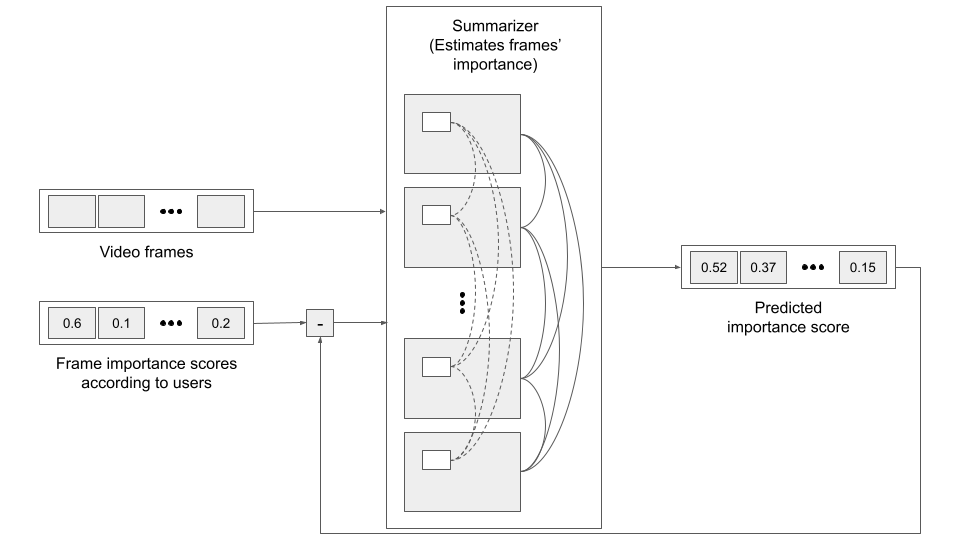
\includegraphics[width=0.73\paperwidth]{content/related/figures/sup-model.png}
  \caption{High-level representation of the analysis pipeline of supervised algorithms that perform summarization by learning the frames' importance after modeling their temporal or spatiotemporal dependency. For the latter class of methods (i.e., modeling the spatiotemporal dependency among frames), object bounding boxes and object relations in time shown with dashed rectangles and lines, are used to illustrate the extension that models both the temporal and spatial dependency among frames.}
  \label{figure:rel-sup-model}
\end{figure}

Early deep-learning-based approaches for video summarization treat the task as a structured prediction problem, aiming to estimate the importance of video frames by modeling their temporal dependencies. During the training phase, these approaches utilize ground-truth data indicating frame importance based on user preferences (see \hyperref[figure:rel-sup-model]{Figure \ref{figure:rel-sup-model}}). The frames' temporal dependencies are modeled, and importance scores are predicted, which are then compared with the ground-truth data to guide the training of the summarization model. 

One of the initial approaches by Zhang \etal~\cite{zhang2016lstm} employed Long Short-Term Memory (LSTM) units to model variable-range temporal dependencies among video frames. Frame importance was estimated using a multi-layer perceptron (MLP), and diversity in the generated summary's visual content was enhanced using Determinantal Point Process (DPP). Zhao \etal~\cite{zhao2017hierarchical} introduced a two-layer LSTM architecture. The first layer extracted and encoded video structure data, while the second layer estimated fragment-level importance and selected key fragments. In their subsequent work, Zhao \etal~\cite{zhao2018hsa} incorporated a component that learned to identify shot-level temporal structure, enabling importance estimation at the shot level and producing a key-shot-based video summary. Extending their method, Zhao \etal~\cite{zhao2020tth} introduced a tensor-train embedding layer to address large feature-to-hidden mapping matrices. This layer, combined with a hierarchical structure of recurrent neural networks (RNNs), captured temporal dependencies within manually-defined video subshots and across different subshots, determining the probability of each subshot being selected for the video summary. Lebron Casas \etal~\cite{lebron2019attention} expanded on the work of Zhang \etal~\cite{zhang2016lstm} by incorporating an attention mechanism to model the temporal evolution of users' interest. This information was then used to estimate frame importance and select keyframes for constructing a video storyboard. Several other methods adopted sequence-to-sequence (seq2seq) architectures with attention mechanisms. Ji \etal~\cite{ji2019attentionEnDe} formulated video summarization as a seq2seq learning problem, using an LSTM-based encoder-decoder network with an intermediate attention layer. They extended their model in Ji \etal~\cite{ji2020deep} by integrating a semantic preserving embedding network and employing the Huber loss instead of Mean Square Error (MSE) loss for enhanced robustness. Fajtl \etal~\cite{fajtl2019summarizing} utilized a soft self-attention mechanism and a two-layer fully connected network for regression to estimate frame importance, avoiding computationally-demanding LSTMs. Liu \etal~\cite{liu2019learning} proposed a hierarchical approach combining a generator-discriminator architecture to estimate shot representativeness and select candidate keyframes, followed by a multi-head attention model for further importance assessment and final keyframe selection. Li \etal~\cite{li2021exploring} introduced a global diverse attention mechanism based on the self-attention mechanism of the Transformer Network, encoding temporal relations between frames and transforming diverse attention weights into importance scores. Another approach, presented by Rochan \etal~\cite{rochan2018sequence}, treated video summarization as a semantic segmentation task, treating the video as a 1D image and employing semantic segmentation models such as Fully Convolutional Networks (FCN) and DeepLab. They developed a network called Fully Convolutional Sequence Network that effectively modeled long-range dependencies among frames and learned frame importance by using convolutions with increasing effective context size. To address the limited capacity of LSTMs, some techniques incorporated additional memory. Feng \etal~\cite{feng2018memory} proposed a deep learning architecture that stored information about the entire video in an external memory, allowing each shot's importance to be predicted by learning an embedding space for matching shots with the memory information. Wang \etal~\cite{wang2019stacked} stacked multiple LSTM and memory layers hierarchically to capture long-term temporal context and estimate frame importance based on this information.